
\subsection{Hadronic Veto System (Editors: Jeremy Mans, Nhan Tran, Andrew Whitbeck)}

The hadronic veto system is designed for detecting rare processes and therefore studies of its performance focus on "bottom up" vetoes of photo-nuclear reactions.  
If we consider that the rare processes described in Section~\ref{} should produce a low multiplicity of neutrons we perform studies to compute on the efficiency the hadronic veto system 
of a detecting single neutron.  
This will give us an idea of the efficiency with which we can veto any type of photo-nuclear reaction based on the hadronic system only.  

We benchmark the hadronic veto system by considering neutrons, being generated at the face of the calorimeter, with various:
\begin{itemize}
\item energies: 1.3, 1.5, 1.8, 2.0, 2.2, 2.5, 3.5~GeV (total energy)
\item number of calorimeter layers: 15, 20, 25
\item incident angles: 0, 15, 30~degrees
\end{itemize}
For each neutron phase space point, we generate $5 \times 10^4$ events.  

First we study the propagation of neutrons through the HCAL purely via {\tt GEANT} without yet considering the digitization of the scintillation signal, which was described in Section~\ref{sec:hcaldig}.
We define the kinetic energy flux for a given layer as the amount of kinetic energy passing through the front face of a given HCAL layer.  
In Fig.~\ref{fig:neturonflux}, we show the neutron kinetic energy flux as a function of HCAL layer for 3.5~GeV total energy neutrons produced at an incident angle of 0.0$^{\circ}$.
We note that the "shower max" for hadronic showers in this system is typically around layers 6/7.  
By looking at the neutron flux around a kinetic energy of 2.5~GeV as a function of layers, we can estimate the fraction of neutrons which pass directly through the calorimeter without interacting.  
We can conclude that roughly $100/50000 \sim 0.2\%$ of neutrons do not interact in the first 15 layers of the system.
This number drops to roughly $0.02\% (0.002\%)$ for a 20 (25) layer system.
This fraction is independent of incident neutron energy.

\begin{figure}[hbtp]
\begin{center}
    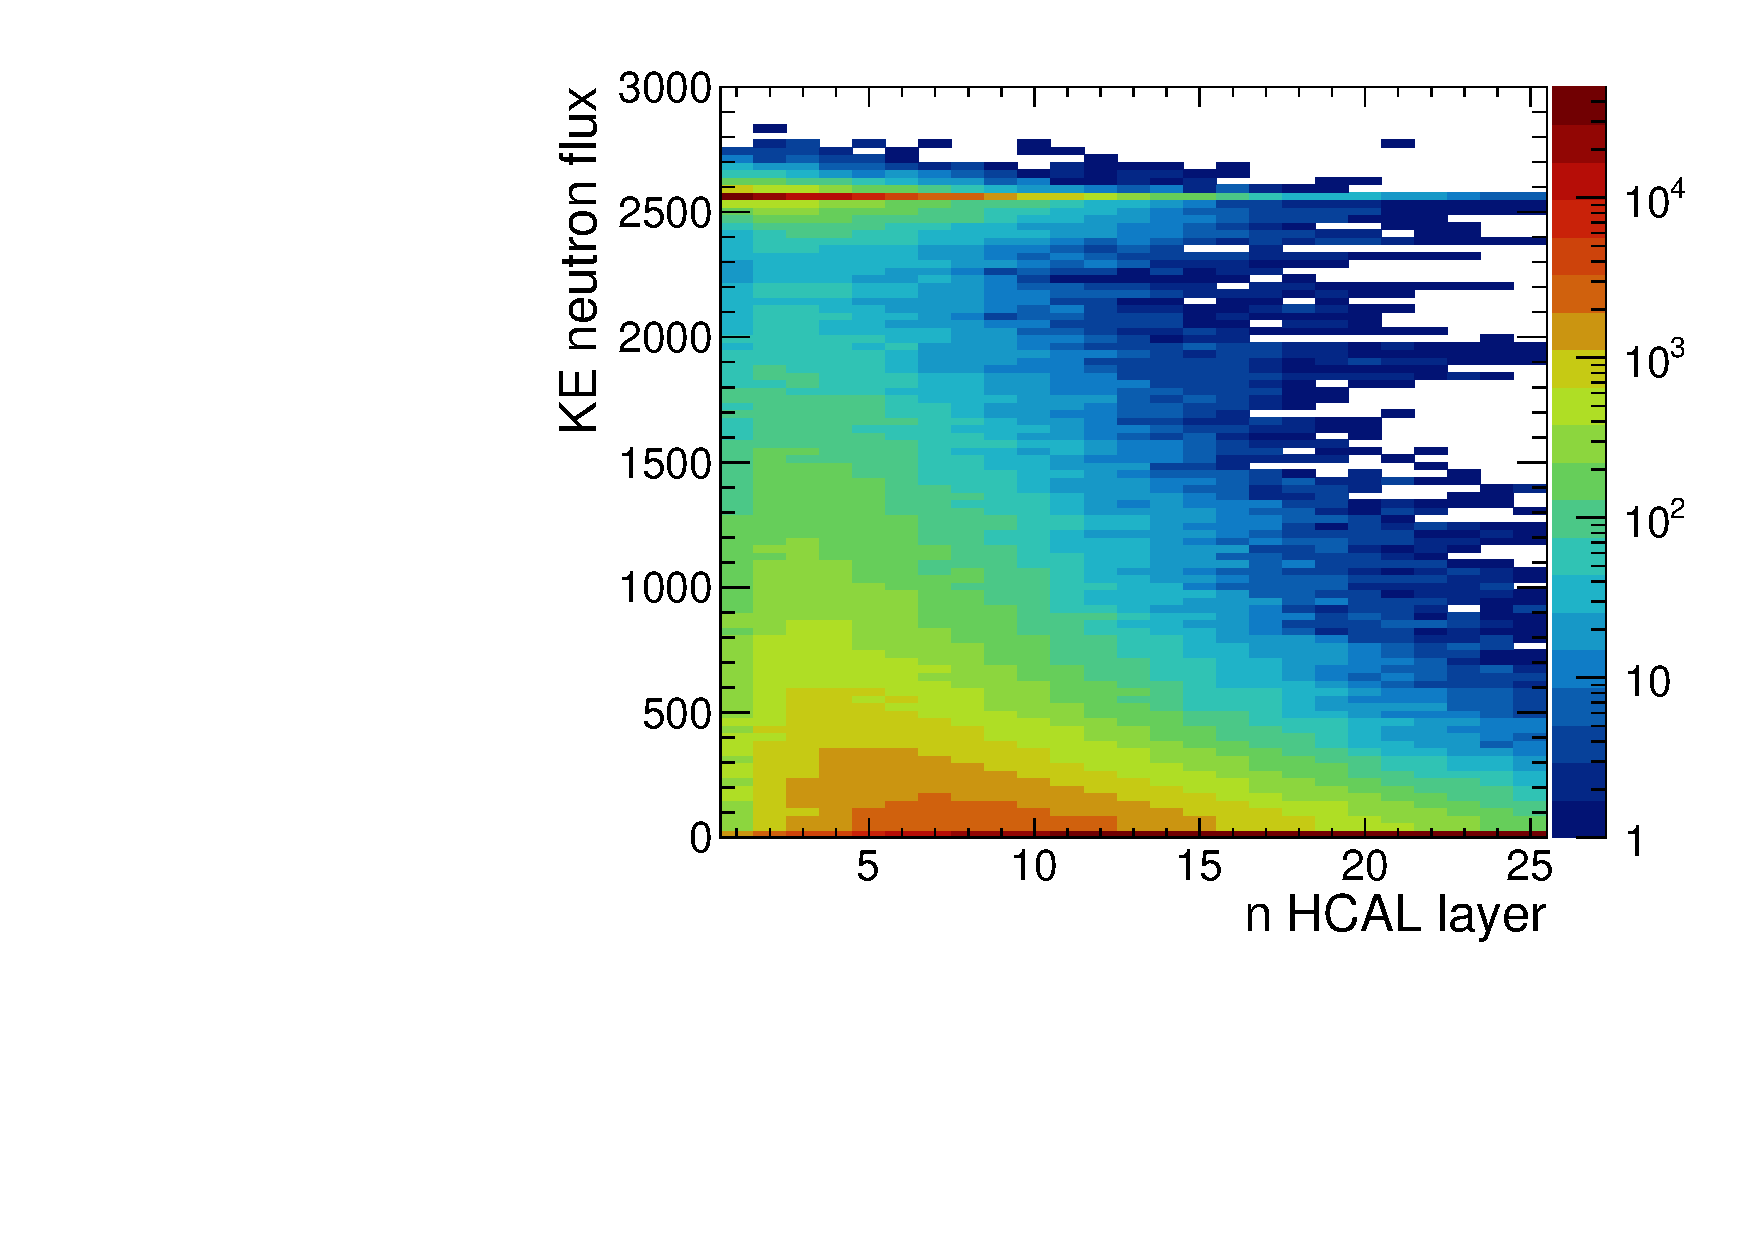
\includegraphics[width=0.5\textwidth]{images/hcal/NFlux_vs_Layer_e3d5_th0d0.pdf}
    \caption{Neutron kinetic energy flux through the HCAL as a function of layer for a 3.5~GeV neutron produced with an incident angle of 0.0$^{\circ}$ at the front face of the calorimeter.}
 \label{fig:neturonflux}
 \end{center}
\end{figure}

For neutrons that do interact in the HCAL, we then compute the efficiency of detecting them given a simple digitization process described in Section~\ref{sec:hcaldig}.
As a reminder, we assume that a MIP deposits, on average, 1.4~MeV of energy in the scintillator, which from CMS testbeam studies we estimate translates into 13.5 photo-electrons at the SiPM.  
Given a typical noise contribution of 2 photo-electrons in SiPMs, we define a MIP signal in a given layer as 8 photo-electrons.  
Therefore, we define a {\it MIP layer} as a scintillator layer in the HCAL in which enough energy is deposited to produce at least 8 photo-electrons (Poisson-varied).   
We define a vetoed neutron event as a neutron which has created $\geq 1$ MIP layer. 
The number of MIP layers is plotted in Fig.~\ref{fig:nmiplayer2d5} for an incident 2.5~GeV total energy neutron assuming a system of 15, 20, or 25 layers; or in other words, counting only MIP layers in the first 15, 20, or 25 HCAL layers (left to right). 
In Fig.~\ref{fig:nmiplayer2d5}, we can count the number of events in the 0 bin of each plot to find the fraction of neutron events which would {\it not} be vetoed, which we call {\it mis-vetoed} neutrons.
For an incident 2.5~GeV total energy neutron, the fraction of mis-vetoed depends strongly on the number of HCAL layers in the system.  
This suggests, for higher energy neutrons, that the mis-veto fraction is dominated by neutrons which do not interact in the system and are not contained.  

\begin{figure}[hbtp]
\begin{center}
    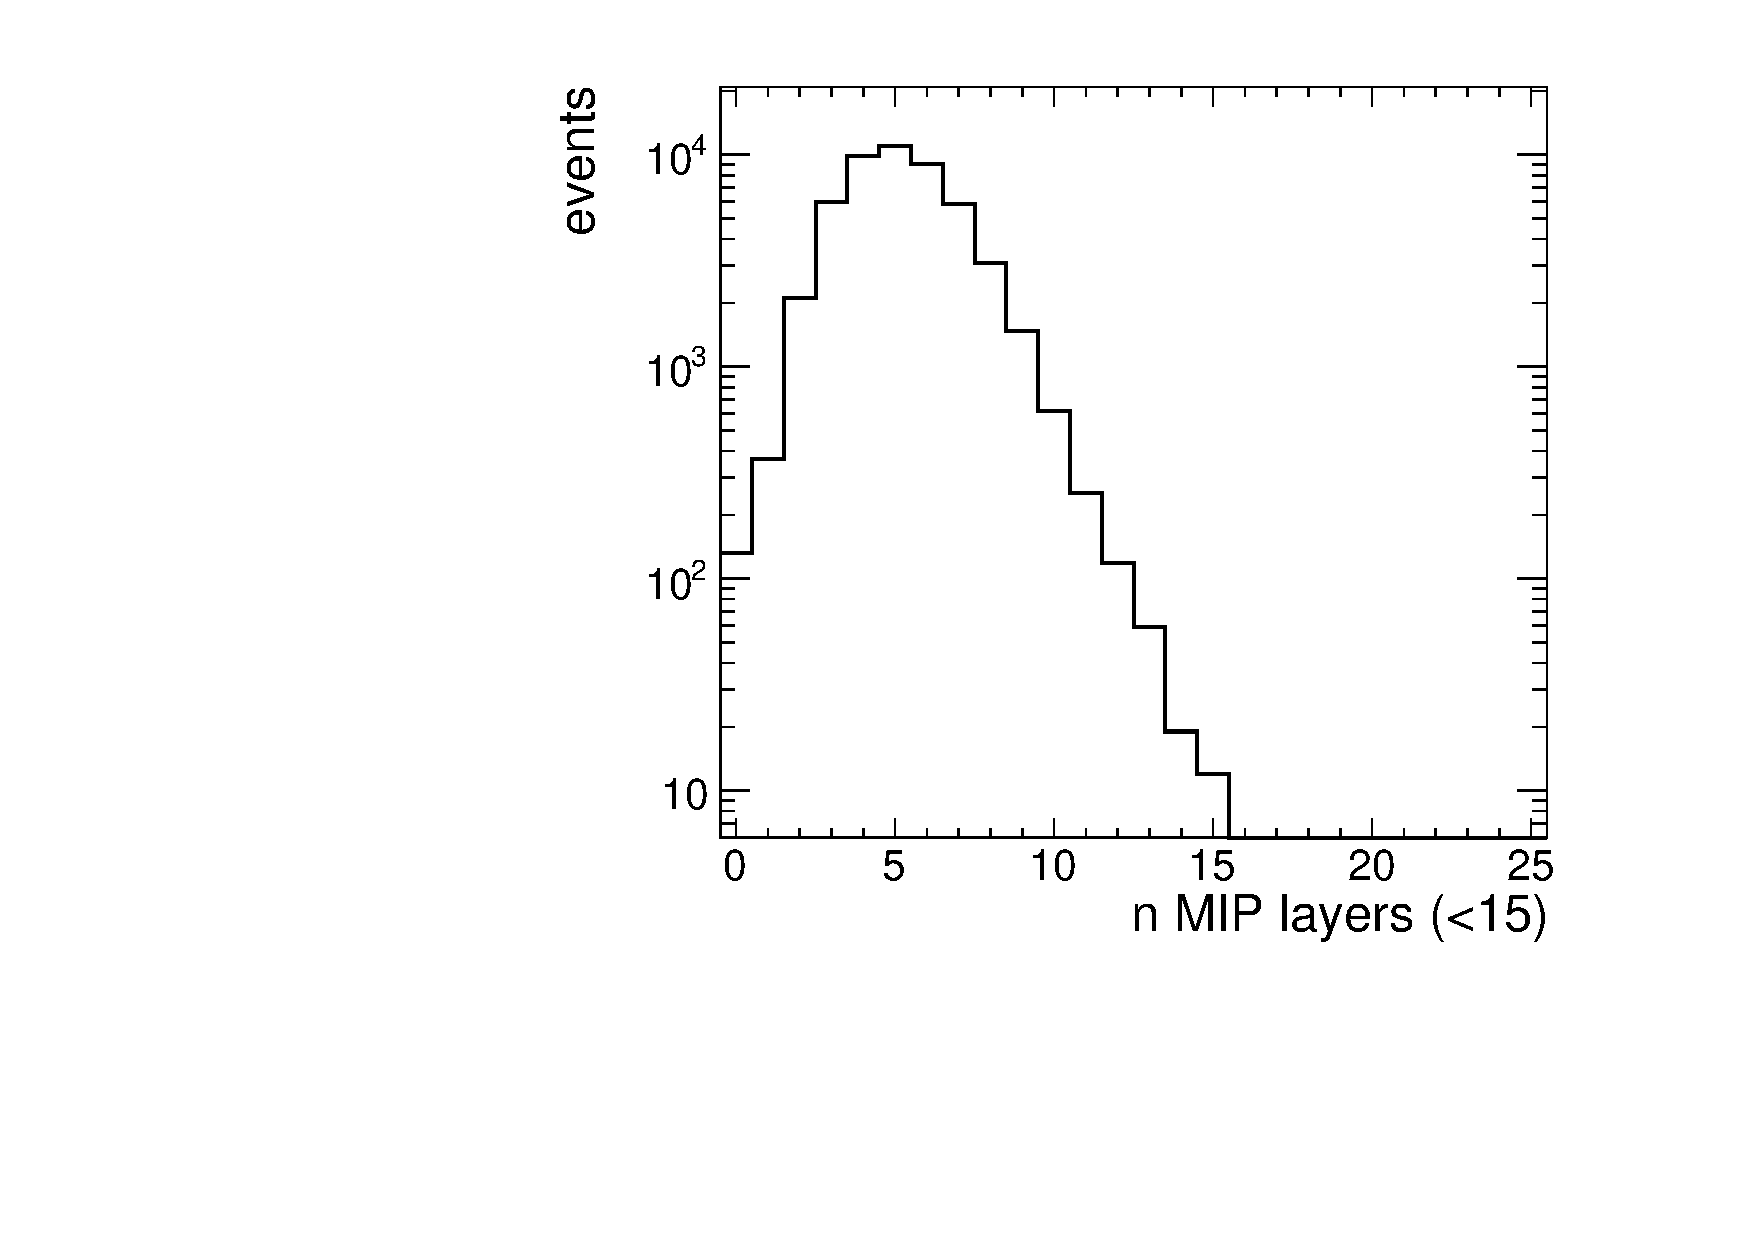
\includegraphics[width=0.3\textwidth]{images/hcal/nMIPLayers15_e2d5.pdf}
    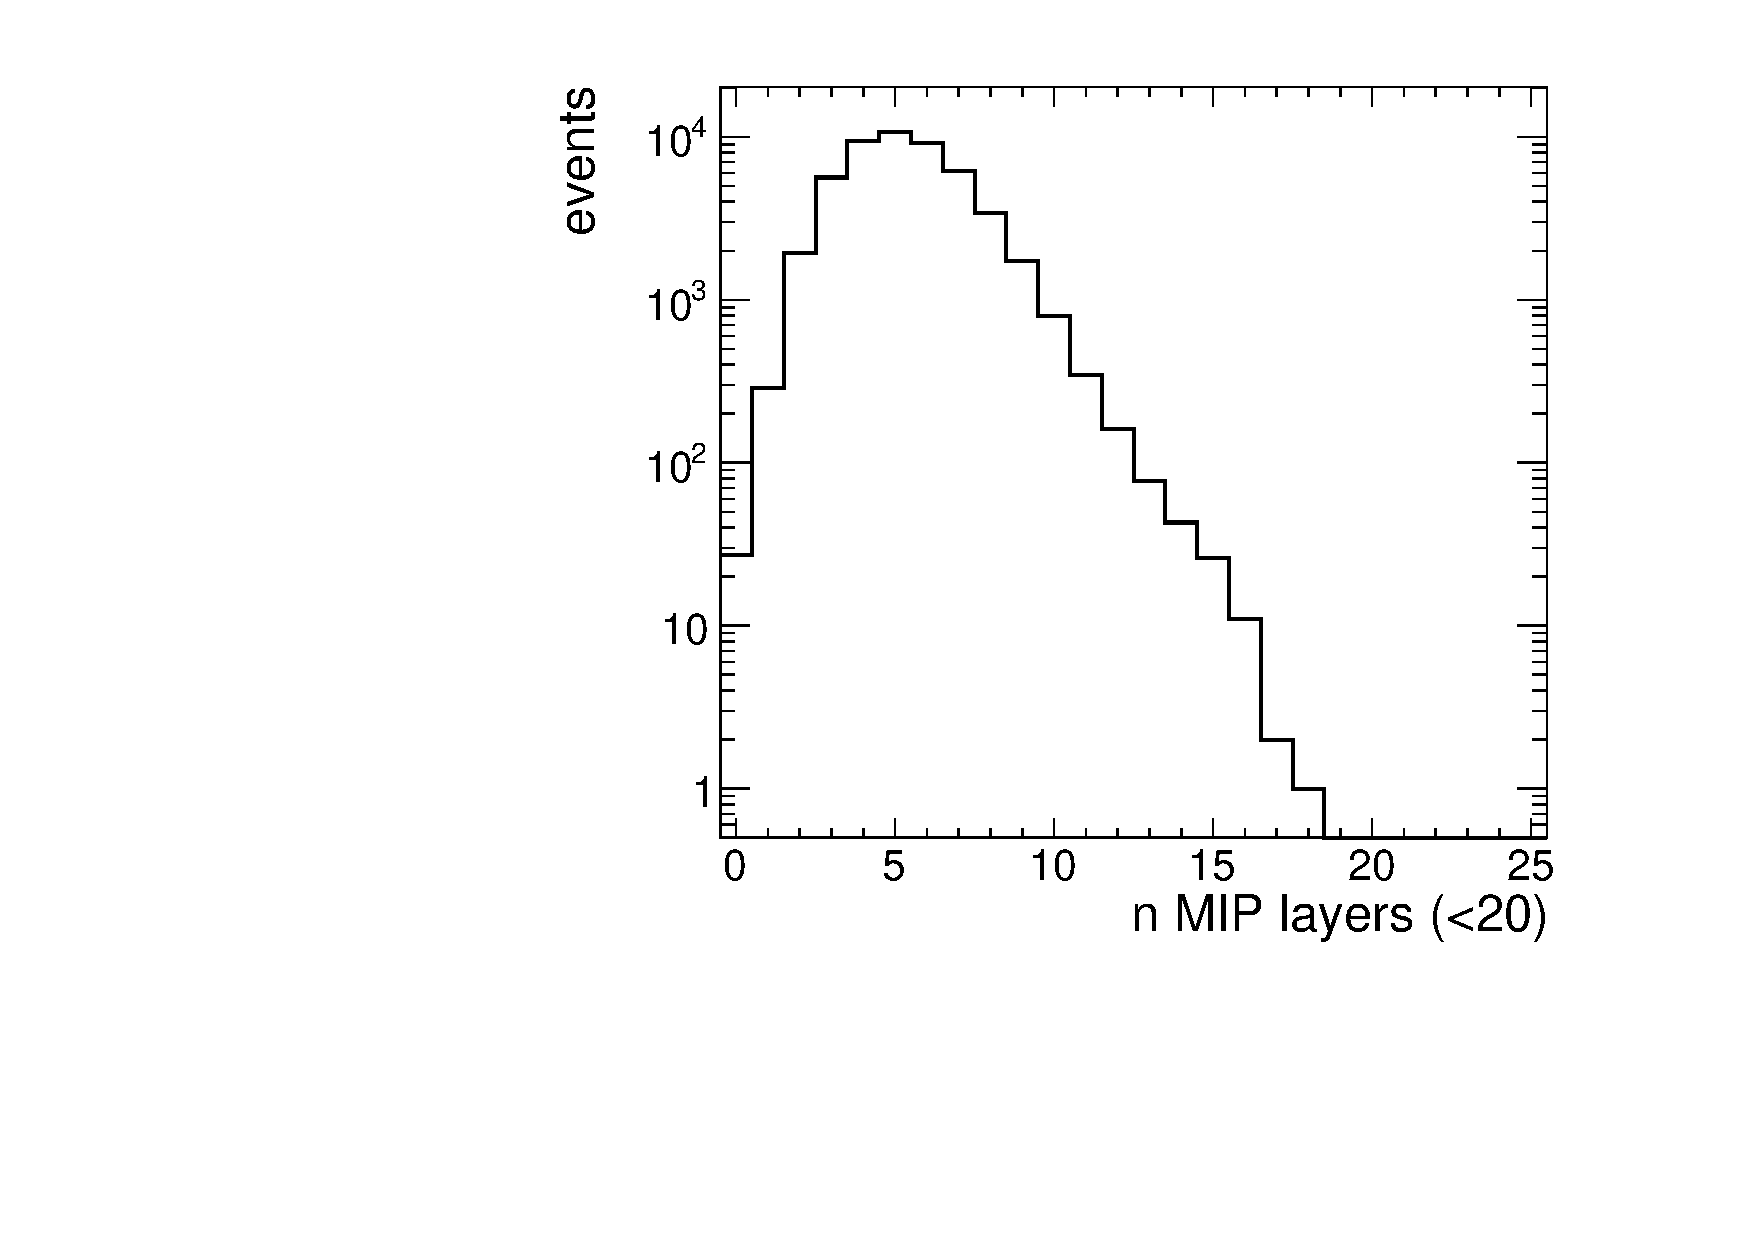
\includegraphics[width=0.3\textwidth]{images/hcal/nMIPLayers20_e2d5.pdf}
    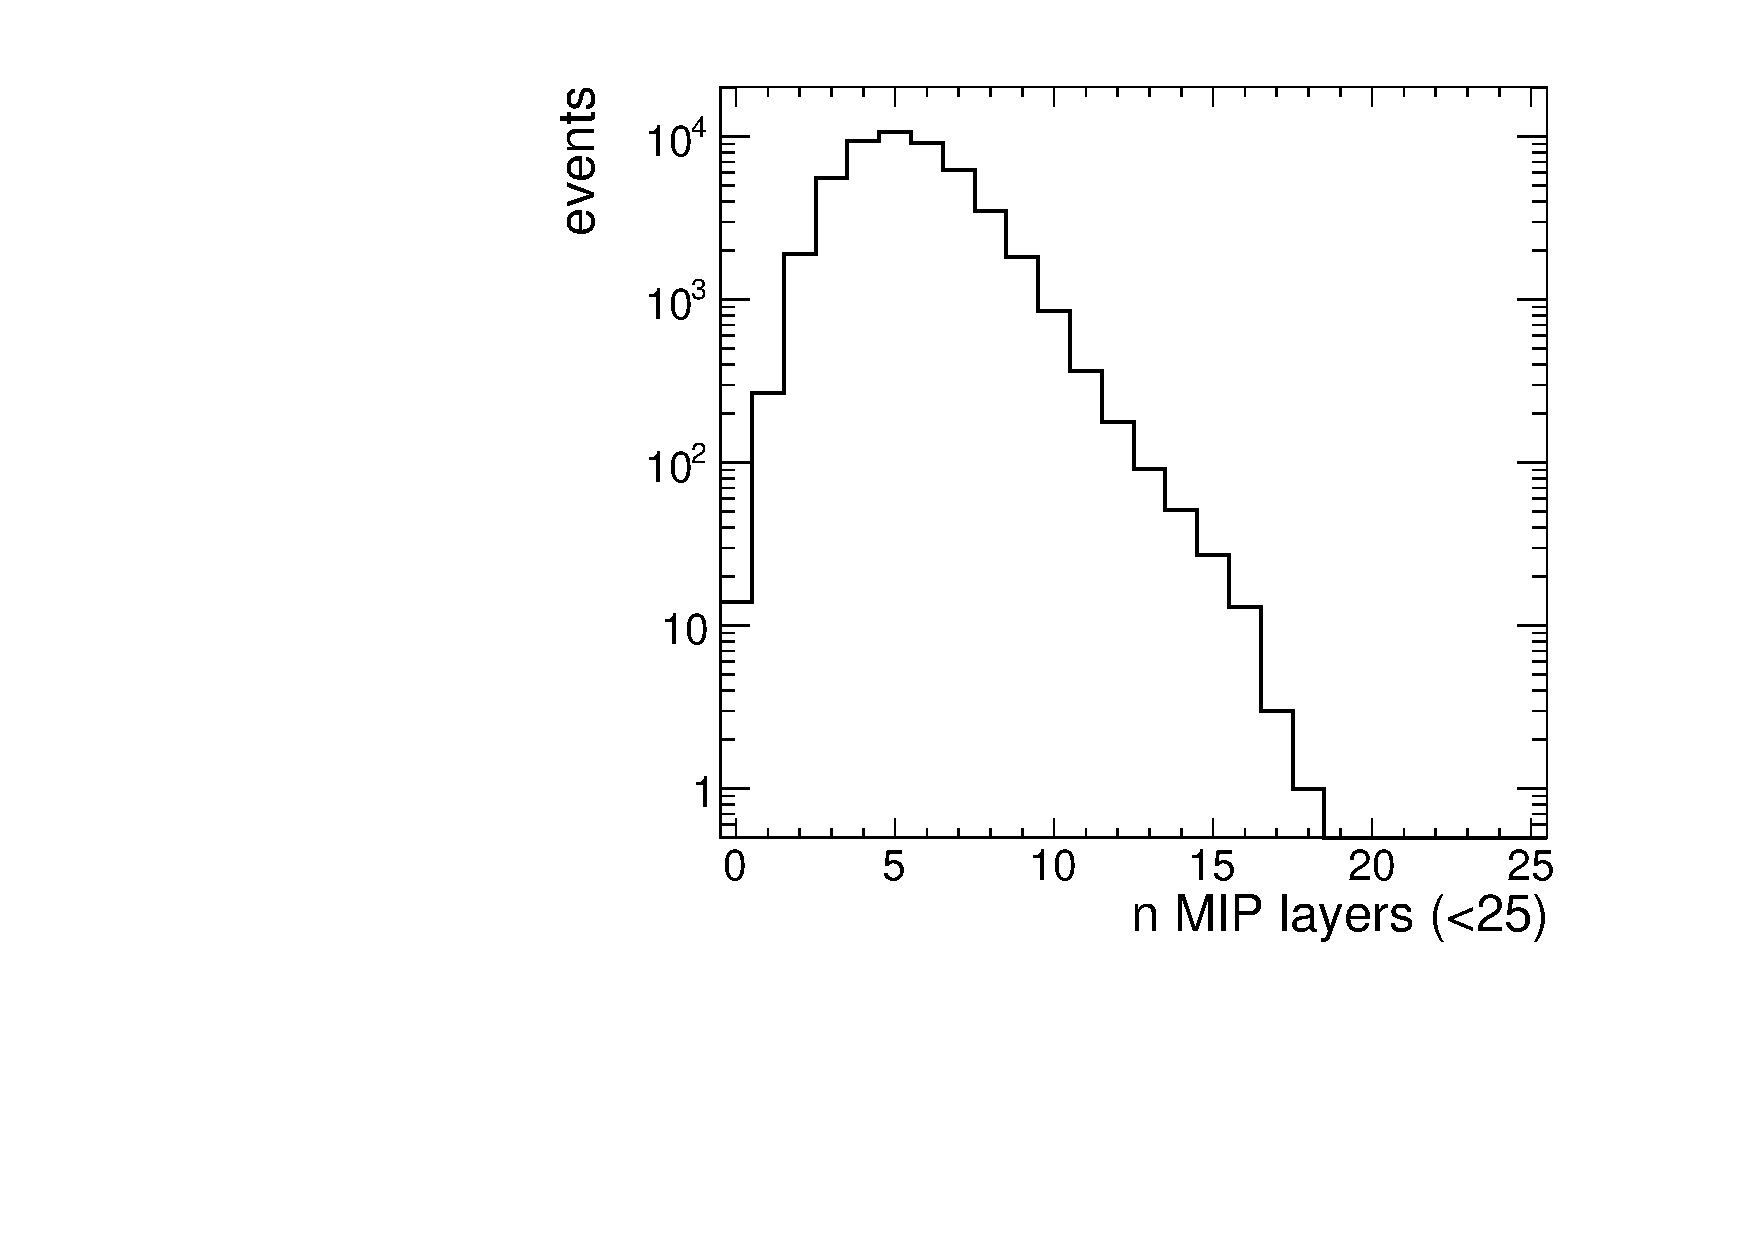
\includegraphics[width=0.3\textwidth]{images/hcal/nMIPLayers25_e2d5.pdf}    
    \caption{Number of MIP layers for a 2.5~GeV neutron produced with an incident angle of 0.0$^{\circ}$ at the front face of the calorimeter for a system of 15, 20, or 25 layers (left to right). }
 \label{fig:nmiplayer2d5}
 \end{center}
\end{figure}

The number of MIP layers is plotted in Fig.~\ref{fig:nmiplayer1d3} for an incident 1.3~GeV total energy neutron assuming a system of 15, 20, or 25 layers (left to right). 
Here, we note that the mis-veto efficiency is fairly constant as a function of the number of HCAL layers in the system.
We conclude that most mis-vetoed neutron events for lower energy neutrons do not deposit enough energy in the scintillator to pass the threshold for a MIP layer or are directly absorbed into the Steel absorber layer.

\begin{figure}[hbtp]
\begin{center}
    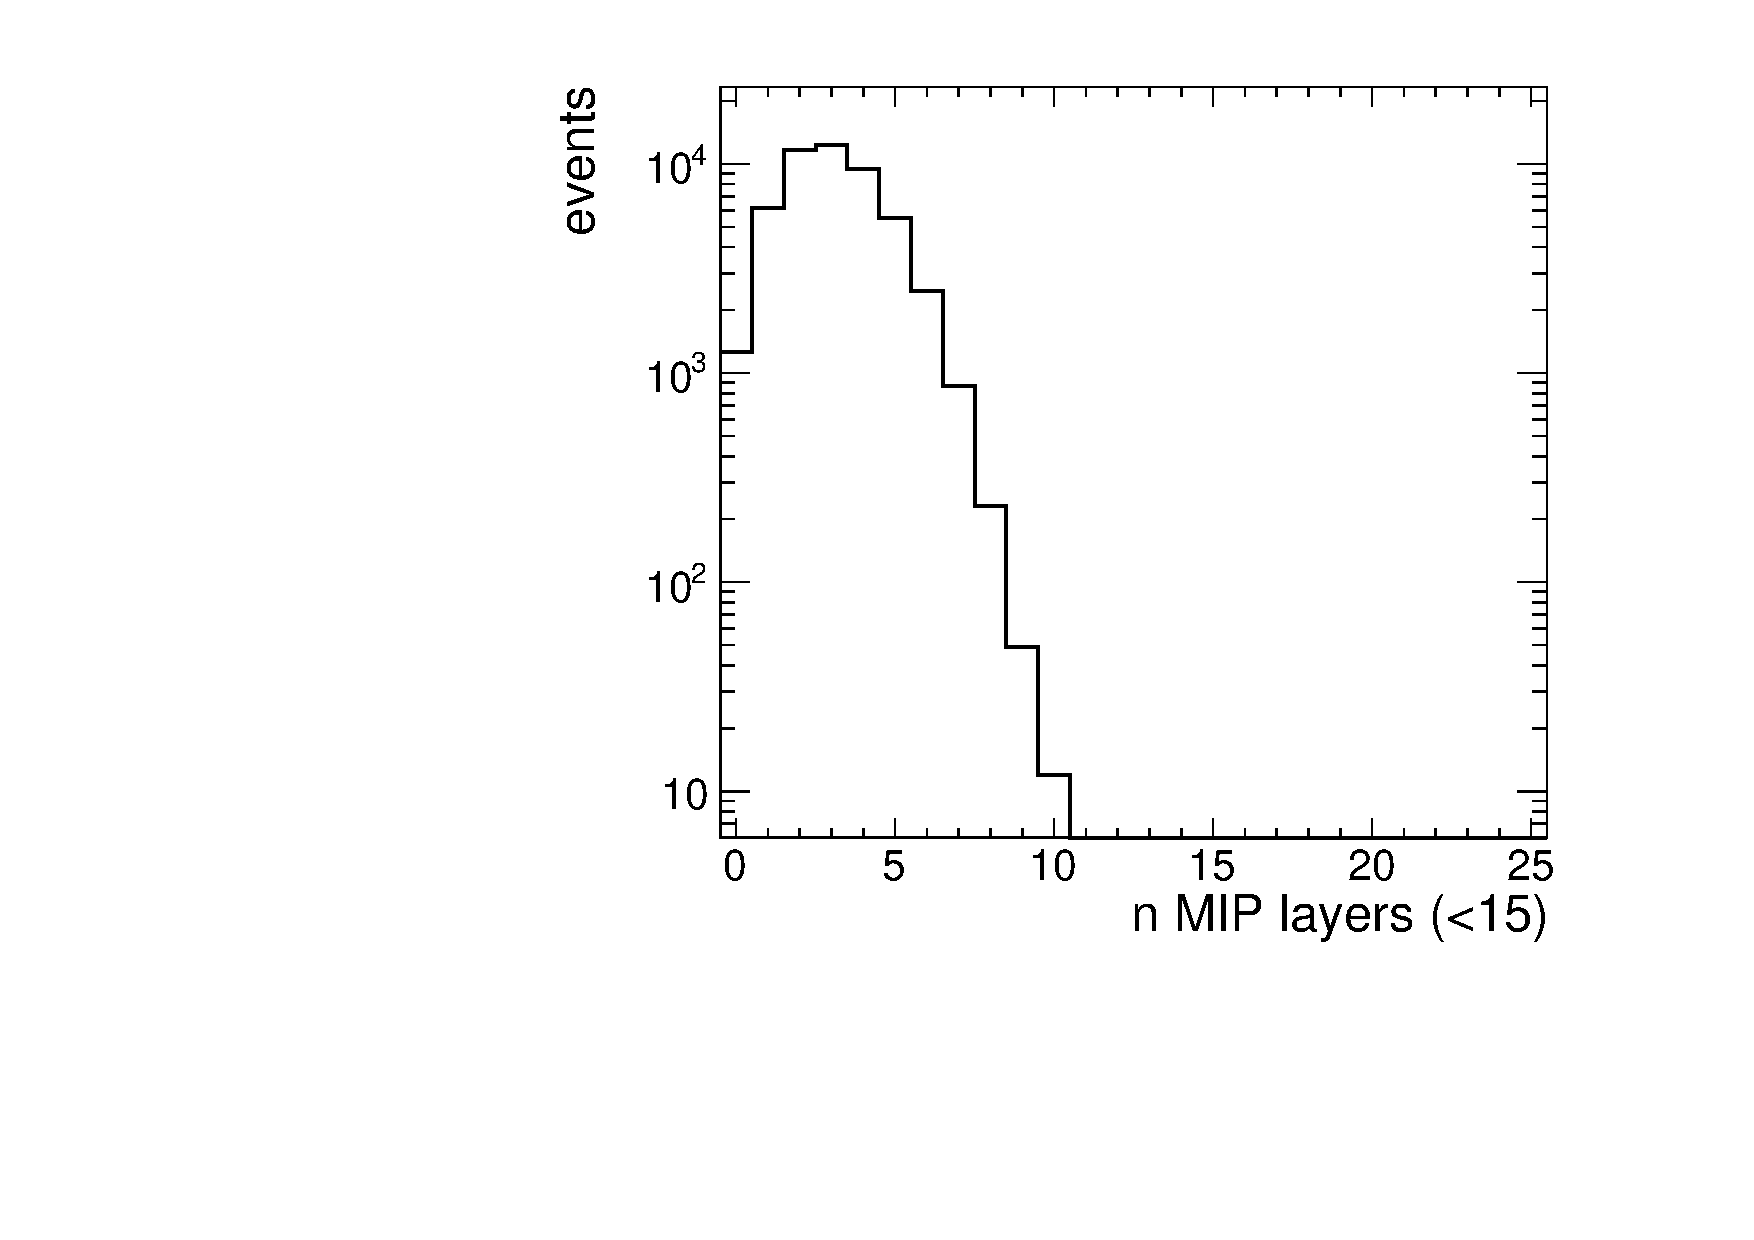
\includegraphics[width=0.3\textwidth]{images/hcal/nMIPLayers15_e1d3.pdf}
    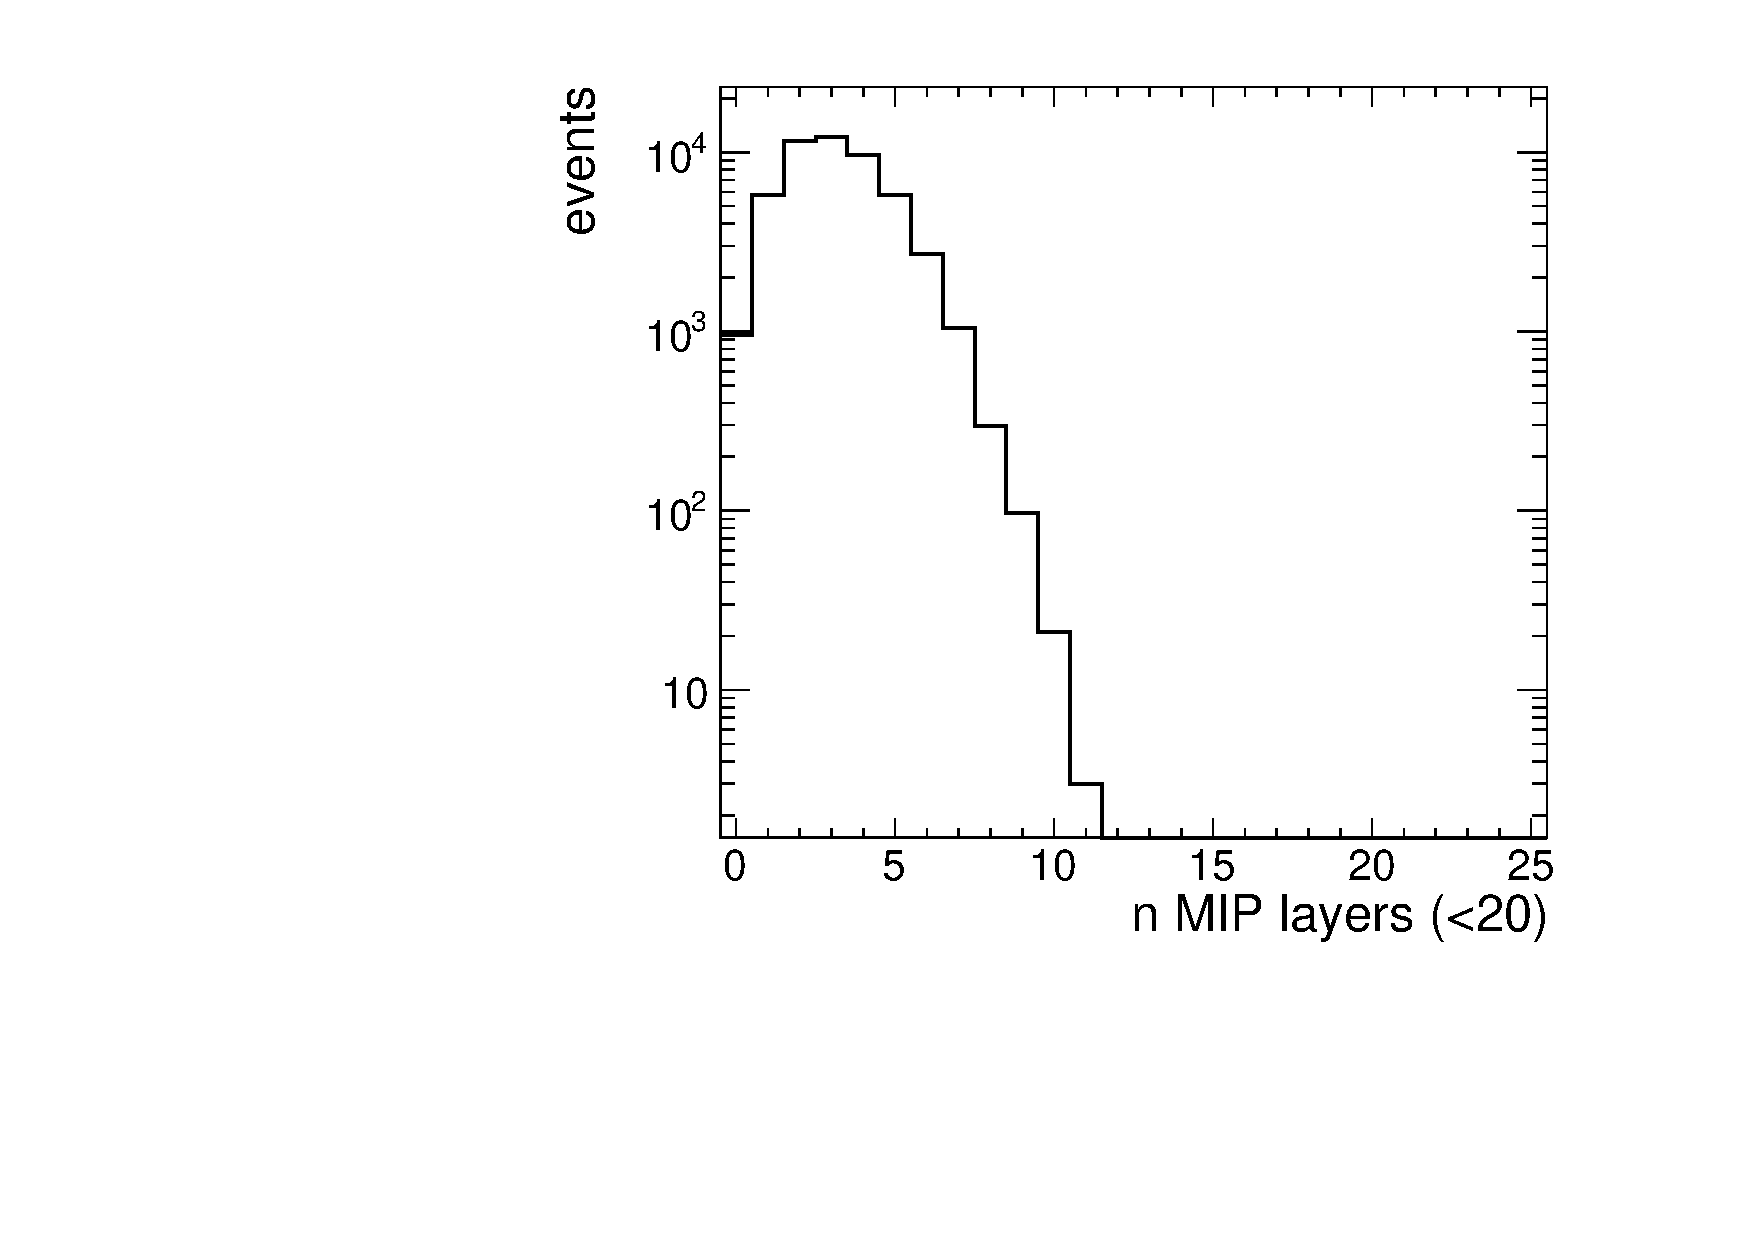
\includegraphics[width=0.3\textwidth]{images/hcal/nMIPLayers20_e1d3.pdf}
    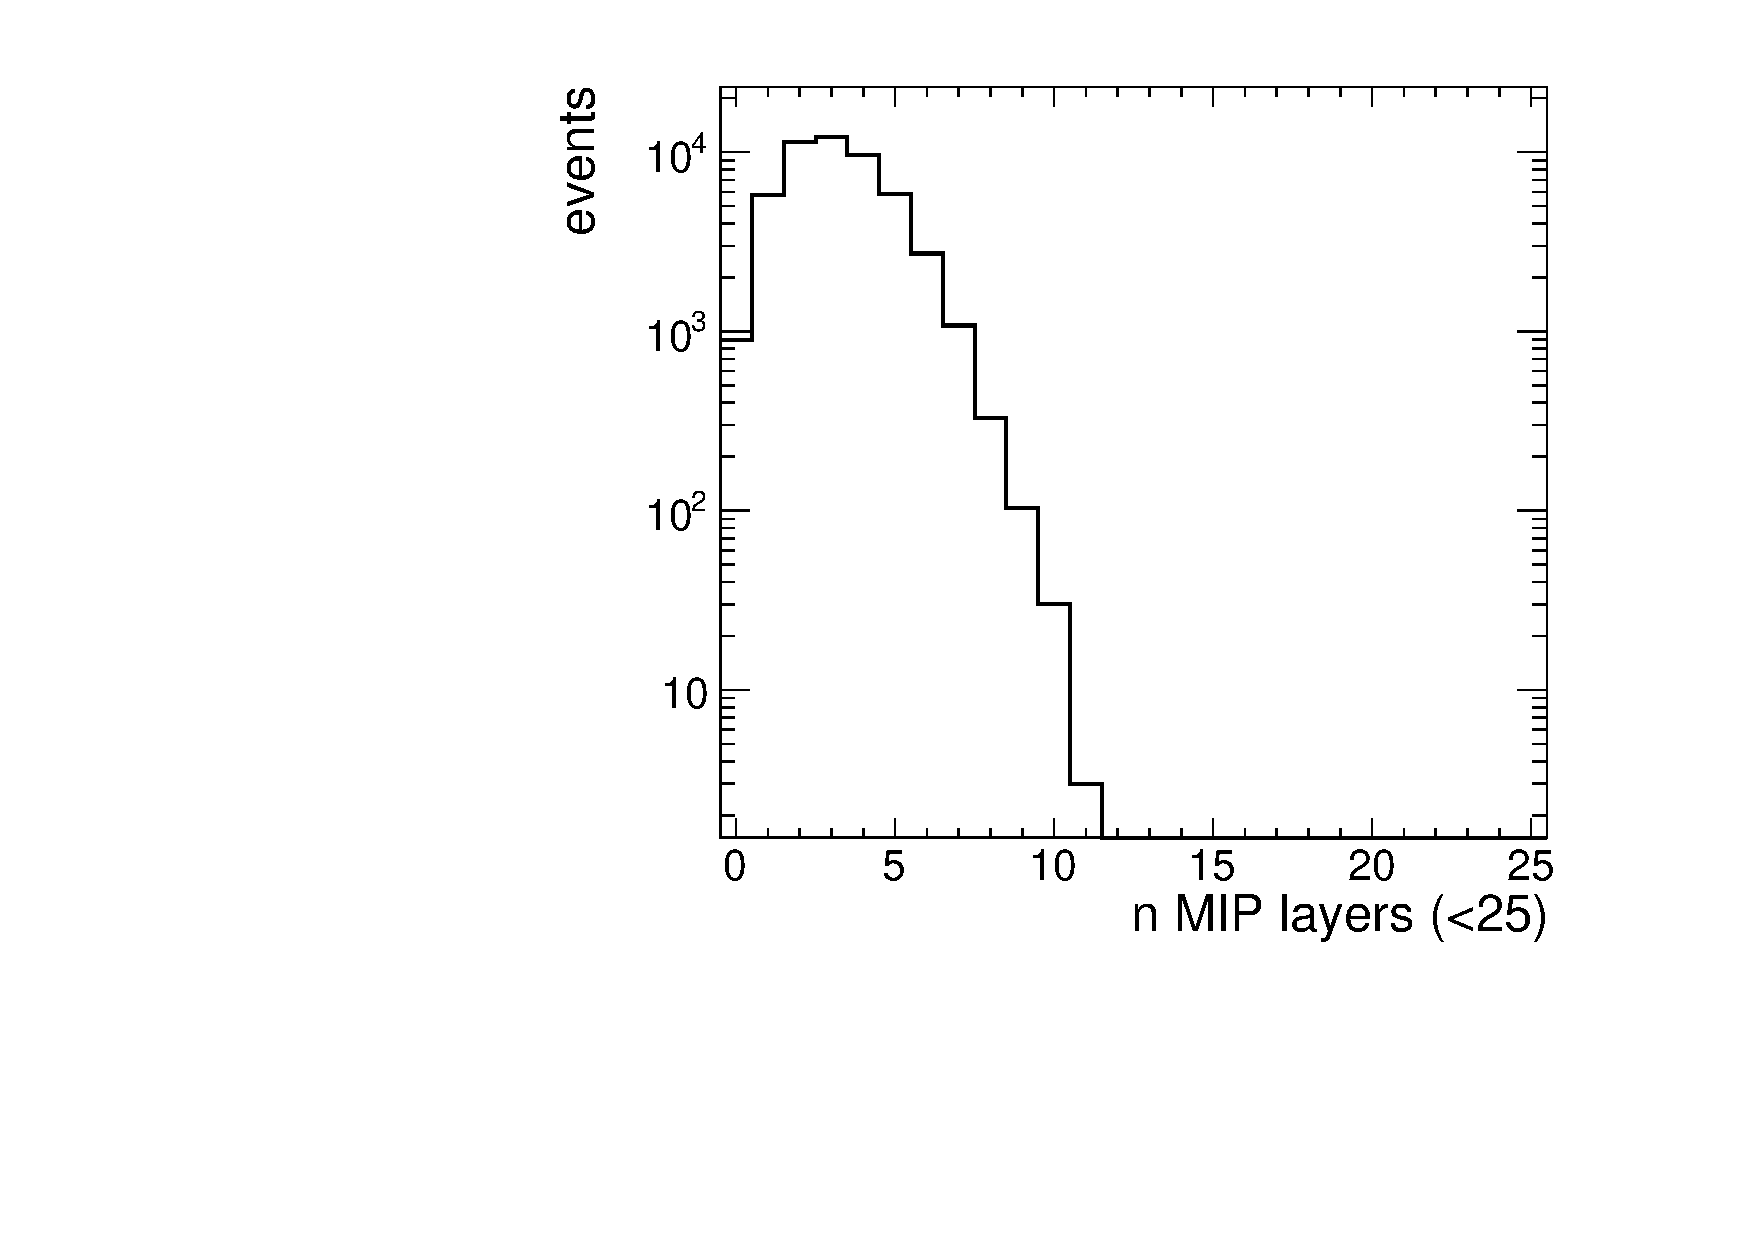
\includegraphics[width=0.3\textwidth]{images/hcal/nMIPLayers25_e1d3.pdf}    
    \caption{Number of MIP layers for a 2.5~GeV neutron produced with an incident angle of 0.0$^{\circ}$ at the front face of the calorimeter for a system of 15, 20, or 25 layers (left to right). }
 \label{fig:nmiplayer1d3}
 \end{center}
\end{figure}

Finally we conclude by benchmarking performance as a function of number of layers in the system and incident neutron angle.
This is shown in Fig.~\ref{fig:effmap1}.
Here we show the neutron mis-veto rate as a function of total energy, incident angle. and number of HCAL layers.  
First we see that the mis-veto rate fall quickly with energy which indicates that we are much more efficient at detecting higher energy neutrons at a mis-veto rate of $10^-3$-$10^-5$ depending on the number of layers in the system and the incident angle of the neutron.  
At higher energies, a larger incident angle or more layers reduces the mis-veto rate where in both cases the neutron traverses more material (absorber).
This indicates that the main source of mis-vetoed neutrons comes neutrons that do not interact with the HCAL.  
For lower energies, the mis-veto rate for neutrons is practically independent of incident angle and number of layers and is typically at a value of $10^-1$.  

\begin{figure}[hbtp]
\begin{center}
    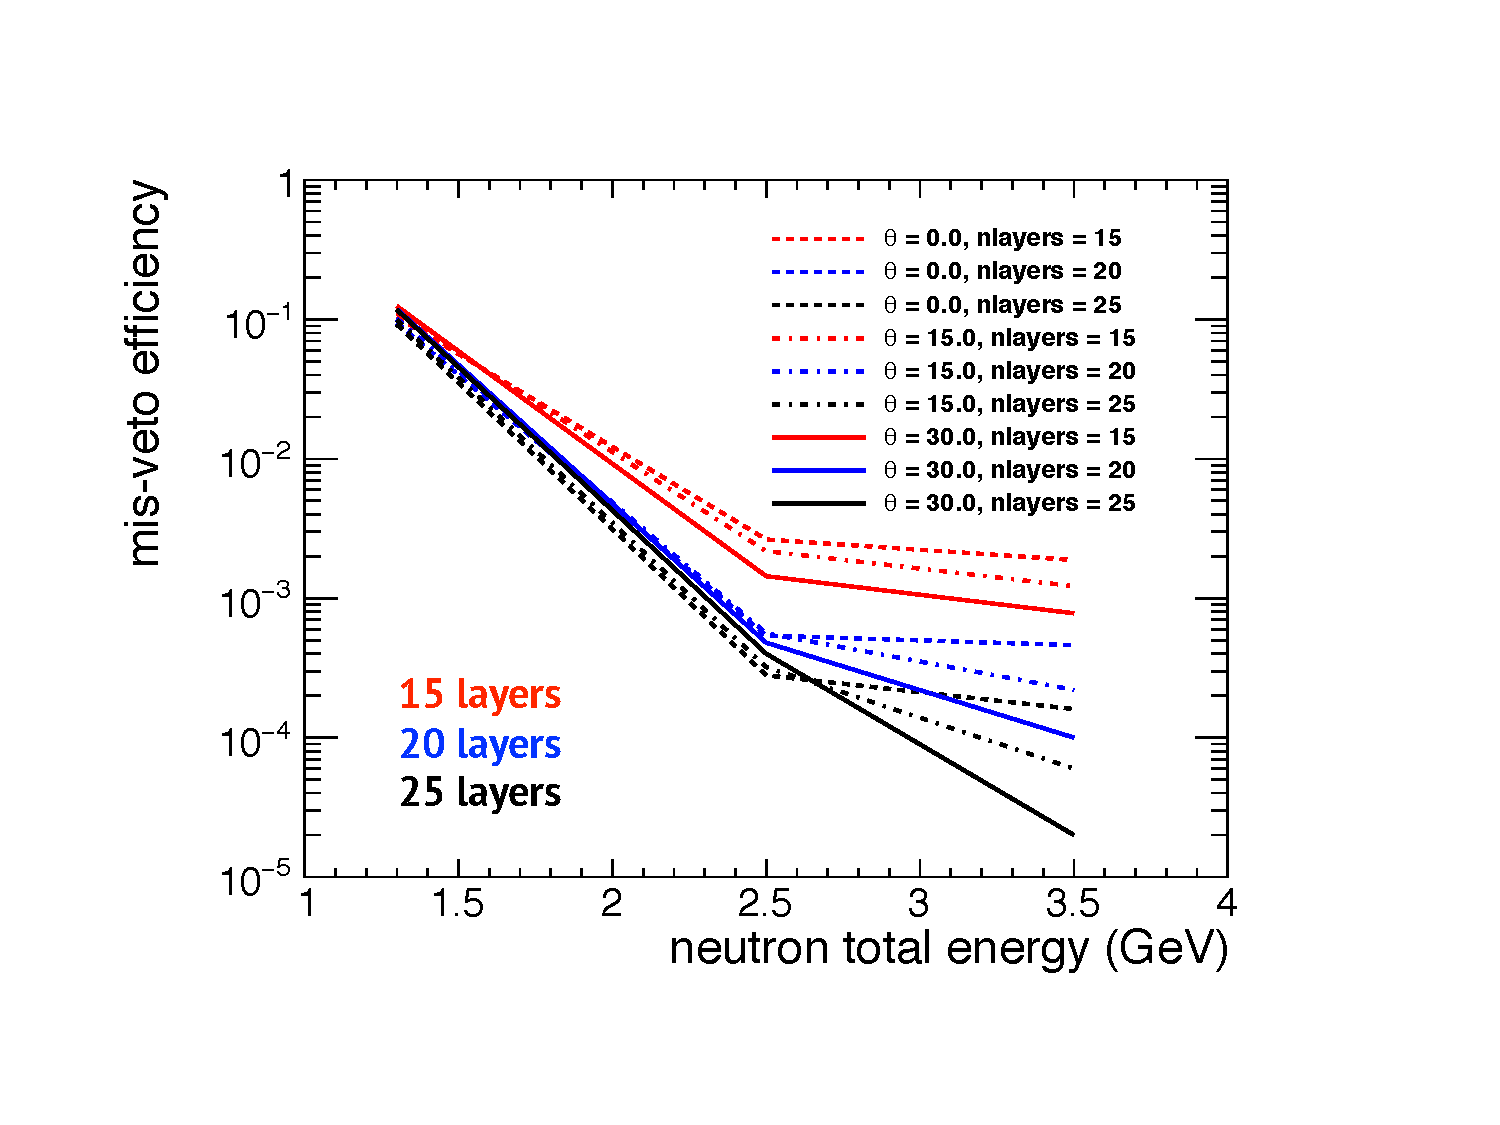
\includegraphics[width=0.6\textwidth]{images/hcal/effmap1.pdf}
    \caption{Number of MIP layers for a 2.5~GeV neutron produced with an incident angle of 0.0$^{\circ}$ at the front face of the calorimeter for a system of 15, 20, or 25 layers (left to right). }
 \label{fig:effmap1}
 \end{center}
\end{figure}

In Fig.~\ref{fig:effmap1}, we show a more fine-grained mis-veto rate plot with more neutron energies considered.

\begin{figure}[hbtp]
\begin{center}
    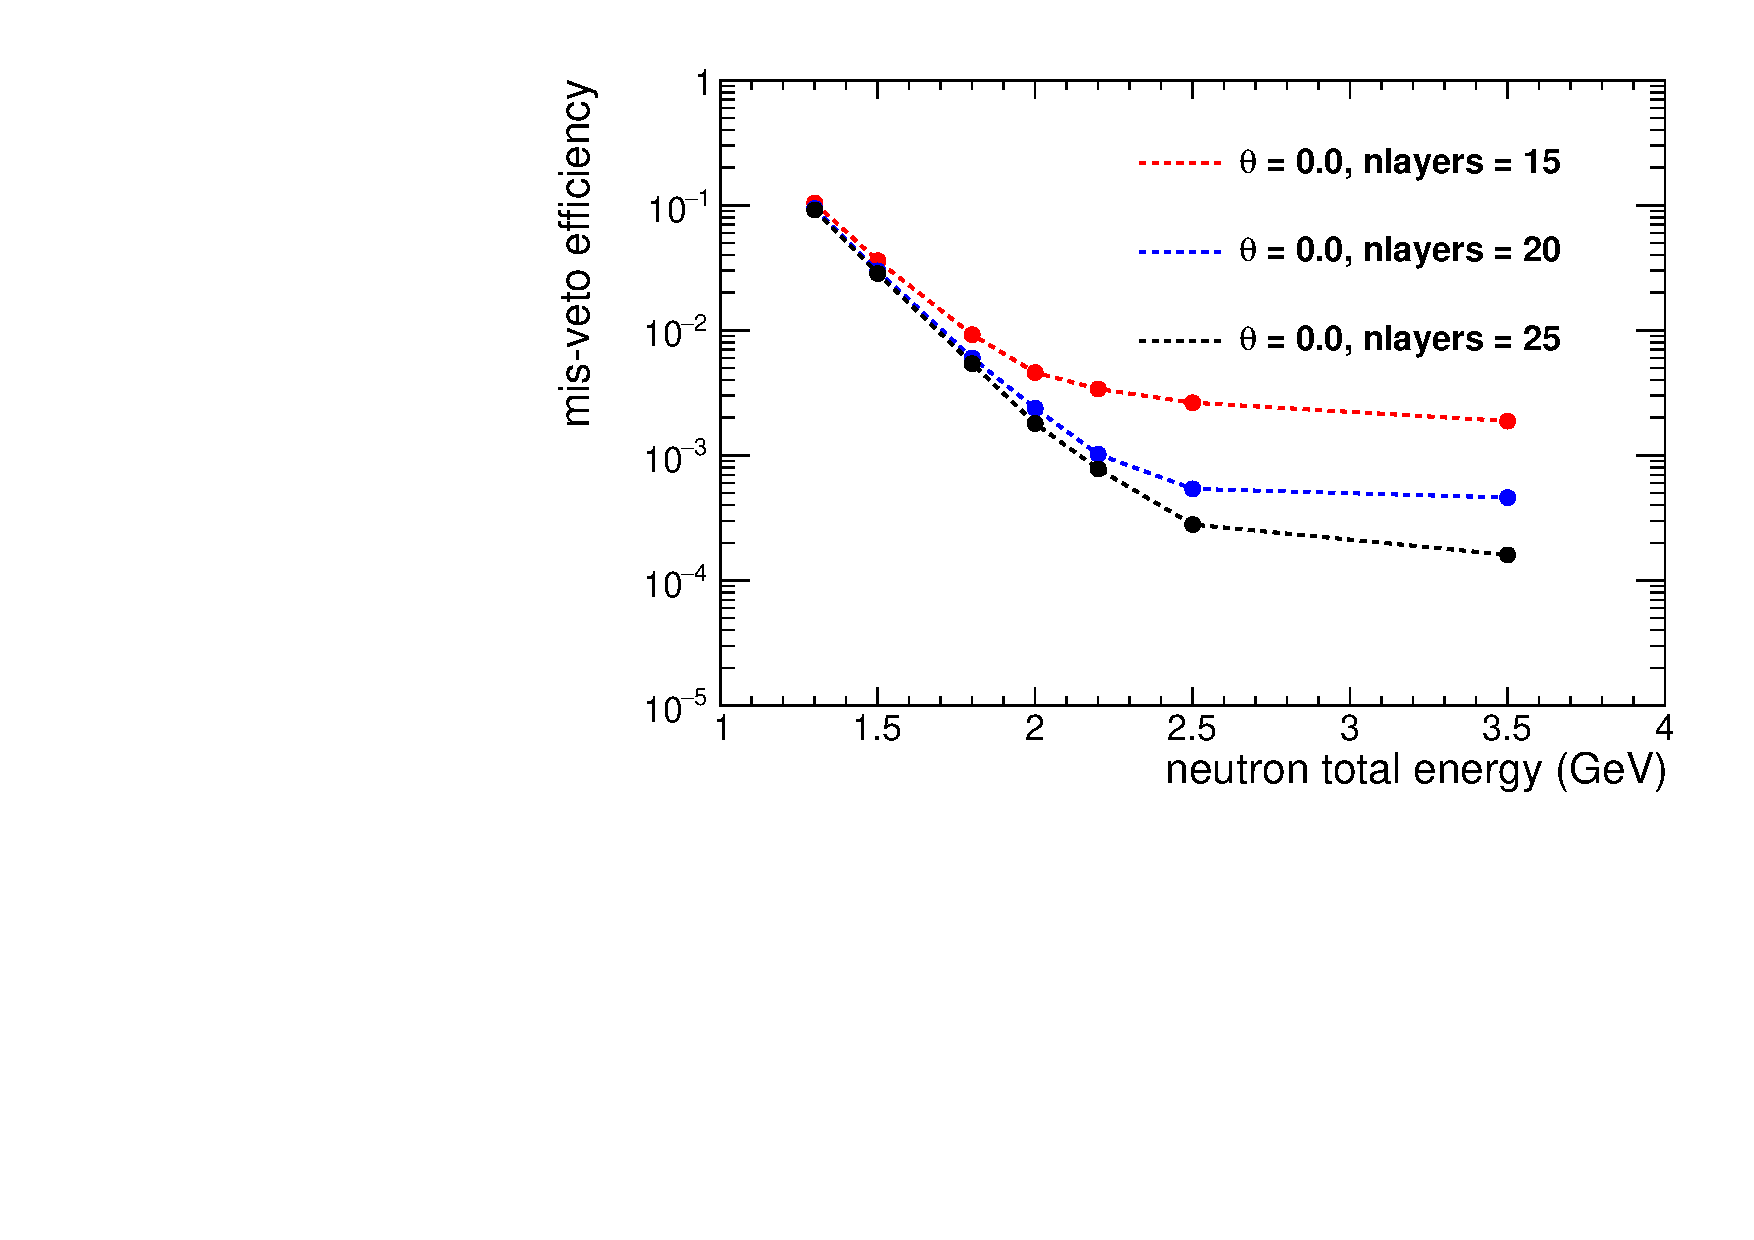
\includegraphics[width=0.6\textwidth]{images/hcal/effmap2.pdf}
    \caption{Number of MIP layers for a 2.5~GeV neutron produced with an incident angle of 0.0$^{\circ}$ at the front face of the calorimeter for a system of 15, 20, or 25 layers (left to right). }
 \label{fig:nmiplayer1d3}
 \end{center}
\end{figure}

%A good starting point would be to focus on the event types that the ECal will certainly have a tough time with. These are the few-body photo-nuclear reactions for sure. So it might make sense to start with the ``bottom up'' study outlined above. 

{\color{red} to add: studies changing absorber thickness and varying MIP layer threshold. Further studies are on-going to better improve performance at lower energies. }

From single neutron studies, we conclude that we are able to veto neutrons at an event per $10^1 - 10^5$ for neutron kinetic energies ranging from 400~MeV to 2.5~GeV 
depending on number of layers in the system and incident angle.  
In the next Section, we study in more detail the veto capabilities of the entire calorimeter system, ECAL + HCAL, for rare photo-nuclear processes.


